\documentclass[12pt,a4paper]{report}

% Core packages for dissertation layout and math
\usepackage[margin=1in]{geometry}
\usepackage{setspace}
\onehalfspacing
\usepackage{amsmath,amssymb,amsthm}
\usepackage{siunitx}
\usepackage{booktabs}
\usepackage{graphicx}
\usepackage{caption}
\usepackage{subcaption}
\usepackage{tikz}
\usepackage{pgfplots}
\pgfplotsset{compat=1.18}
\usepackage[numbers,sort&compress]{natbib}
\usepackage{hyperref}
\usepackage[nameinlink,noabbrev]{cleveref}
\usepackage{longtable}
\usepackage{array}
\usepackage{multirow}
\usepackage{enumitem}

\hypersetup{colorlinks=true,linkcolor=blue,citecolor=blue,urlcolor=blue}

% Dissertation metadata
\title{Enhancing the Efficiency of Thermoelectric Systems Using Phase Change Materials Embedded within Hierarchical Nanoporous Polyvinyl Alcohol (PVA) Scaffolds Reinforced with CuS--MoS$_2$ Nanostructures}
\author{Candidate Name}
\date{\today}

\begin{document}

\begin{titlepage}
    \centering
    {\Large University Name\\[1.0cm]}
    {\large Faculty of Engineering and Applied Sciences\\[0.5cm]}
    {\large Department of Materials and Energy Systems\\[1.5cm]}
    {\Huge\bfseries Enhancing the Efficiency of Thermoelectric Systems Using Phase Change Materials Embedded within Hierarchical Nanoporous Polyvinyl Alcohol (PVA) Scaffolds Reinforced with CuS--MoS$_2$ Nanostructures\\[1.5cm]}
    {\Large A Dissertation Submitted in Partial Fulfillment of the Requirements for the Degree of Doctor of Philosophy\\[1.5cm]}
    {\large by\\[0.2cm] Candidate Name\\[1.0cm]}
    {\large Supervisor: Prof. Supervisor Name\\[2.0cm]}
    {\large \today}
\end{titlepage}

\pagenumbering{roman}

\chapter*{Abstract}
\addcontentsline{toc}{chapter}{Abstract}
Thermoelectric systems provide solid-state heat-to-electricity conversion with high reliability and low maintenance; however, widespread deployment remains constrained by modest conversion efficiencies under fluctuating thermal boundary conditions. This dissertation develops and evaluates a hybrid thermal-electrical material architecture in which a phase change material (PCM) is embedded inside a \emph{hierarchical nanoporous polyvinyl alcohol (PVA) scaffold} that is reinforced by dispersed CuS--MoS$_2$ nanostructures. A central constraint, maintained throughout this work, is that PVA is the sole continuous scaffold matrix. CuS--MoS$_2$ acts strictly as a reinforcing nanofiller within the PVA network and does not replace, coat over, or become the scaffold framework. The PCM is infiltrated into porosity engineered into PVA via freeze-drying and post-crosslink stabilization. This configuration is designed to buffer transient heat, improve thermal contact regularity at the thermoelectric interface, and increase useful temperature gradients over realistic duty cycles.

The study establishes a coupled multiphysics framework linking thermoelectric transport, phase-transition thermodynamics, and scaffold-scale effective transport. The theoretical chapters derive Seebeck, Peltier, and Thomson relations from irreversible thermodynamics and Onsager coupling, then formalize the figure of merit $ZT = S^2\sigma T/\kappa$ with decomposition $\kappa=\kappa_e+\kappa_l$, including deviations from the Wiedemann--Franz law in nanostructured composites. A latent-heat enthalpy formulation and Stefan-interface interpretation are integrated with transient conduction in porous domains. The PVA chapter quantifies hydrogen-bond-mediated mechanics, crystallinity effects, pore hierarchy control, and confinement constraints for leakage-resistant PCM retention under thermal cycling. The CuS--MoS$_2$ chapter models reinforcement-driven percolation, interfacial (Kapitza) resistance, and phonon boundary scattering, while preserving the PVA-continuous topology.

A synthetic but physically constrained case study demonstrates that a properly tuned PVA/PCM/CuS--MoS$_2$ architecture can reduce peak thermal fluctuation amplitude, suppress entropy generation hot-spots, and improve exergy efficiency relative to unbuffered baselines. Parameter sweeps identify optimal pore volume fraction, filler loading below agglomeration threshold, and PCM melting range alignment with source transients. Proposed validation pathways include differential scanning calorimetry (DSC), scanning electron microscopy (SEM), electrical conductivity and thermal conductivity testing, and uncertainty propagation from measurement noise into predicted efficiency metrics.

The dissertation contributes: (i) a defense-level integrated theory for thermoelectric enhancement under transient forcing, (ii) a materials architecture that explicitly separates scaffold function (PVA), reinforcement function (CuS--MoS$_2$), and latent storage function (PCM), and (iii) design maps translating multiphysics parameters into experimentally actionable targets. Limitations and future work are detailed, including long-duration durability, humidity effects on PVA, and scale-up manufacturing pathways for module-level implementation.

\chapter*{Acknowledgments}
\addcontentsline{toc}{chapter}{Acknowledgments}
I express deep gratitude to my supervisor, committee members, laboratory colleagues, and family for their sustained support. Their scientific feedback, technical mentorship, and encouragement made this dissertation possible. I also acknowledge the institutional facilities that enabled conceptual modeling and prototype planning.

\tableofcontents
\listoffigures
\listoftables

\chapter*{Nomenclature and List of Symbols}
\addcontentsline{toc}{chapter}{Nomenclature and List of Symbols}
\begin{longtable}{>{\raggedright\arraybackslash}p{3cm}p{10cm}}
\toprule
Symbol & Description \\
\midrule
$S$ & Seebeck coefficient \\
$\Pi$ & Peltier coefficient \\
$\tau$ & Thomson coefficient \\
$\sigma$ & Electrical conductivity \\
$\kappa$ & Thermal conductivity \\
$\kappa_e,\kappa_l$ & Electronic and lattice thermal conductivity components \\
$ZT$ & Dimensionless thermoelectric figure of merit \\
$T$ & Absolute temperature \\
$q$ & Heat flux \\
$\mathbf{J}_e$ & Electrical current density \\
$L$ & Latent heat of PCM \\
$f_l$ & Liquid fraction of PCM \\
$R_K$ & Kapitza interfacial thermal resistance \\
$\phi_p$ & Pore volume fraction in PVA scaffold \\
$\phi_f$ & CuS--MoS$_2$ filler volume fraction \\
$\eta_{ex}$ & Exergy efficiency \\
\bottomrule
\end{longtable}

\clearpage
\pagenumbering{arabic}

\chapter{Introduction}\label{ch:intro}

Thermoelectric conversion is attractive for distributed power generation, waste heat recovery, and thermal regulation because it uses solid-state modules with no moving parts \citep{bell2008cooling,snyder2008complex}. Yet practical operation often occurs under time-varying heat loads, causing unstable temperature gradients and suboptimal conversion efficiency. This dissertation addresses that transient bottleneck through a materials architecture in which a phase change material is embedded in a \textbf{hierarchical nanoporous PVA scaffold} reinforced with CuS--MoS$_2$ nanofillers.

\section{Research Gap and Problem Statement}
Three gaps motivate this work. First, most thermoelectric optimization studies emphasize static $ZT$ enhancement while neglecting transient thermal buffering \citep{he2017advances}. Second, PCM-integrated thermal management frequently uses metallic or ceramic matrices with limited flexibility and high interfacial mismatch \citep{zhang2020pcmreview}. Third, composite studies can ambiguously attribute scaffold function to fillers. In this dissertation, the scaffold is strictly PVA, CuS--MoS$_2$ only reinforces PVA, and PCM is confined inside PVA porosity.

The governing challenge is maximizing net electrical output under fluctuating thermal sources while minimizing entropy generation and mechanical degradation across cycles.

\section{Objectives}
The main objective is to establish and validate a design framework for PVA/PCM/CuS--MoS$_2$ thermoelectric coupling. Sub-objectives include:
\begin{enumerate}[label=(\roman*)]
    \item formulate coupled transport and phase-change equations,
    \item design hierarchical pore architecture for PCM confinement,
    \item quantify filler-driven transport enhancement without violating scaffold continuity,
    \item evaluate exergy and irreversibility metrics under cycling.
\end{enumerate}

\section{Novelty}
The explicit novelty is the tri-functional separation of roles:
\begin{itemize}
    \item \textbf{PVA:} continuous mechanical scaffold and porous host,
    \item \textbf{PCM:} latent thermal buffer within PVA pores,
    \item \textbf{CuS--MoS$_2$:} reinforcing nanofillers to tune conductivity and interfaces.
\end{itemize}

\begin{equation}\label{eq:intro_power_balance}
\dot{W}_{net}=\int_{A}\left(S\,\Delta T\right)\,\mathrm{d}I-\dot{Q}_{loss},
\end{equation}
where thermal buffering reduces $\dot{Q}_{loss}$ during high-frequency fluctuations.

\begin{figure}[htbp]
\centering
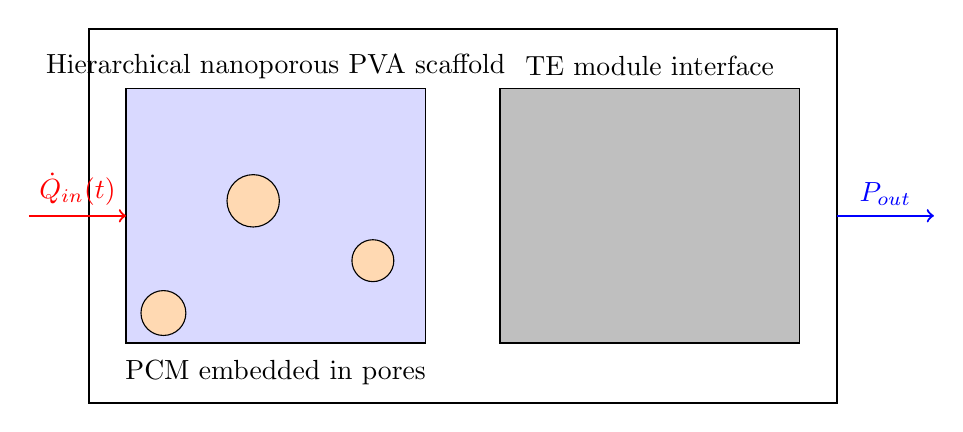
\begin{tikzpicture}[scale=0.95]
\draw[thick] (0,0) rectangle (10,5);
\draw[fill=blue!15] (0.5,0.8) rectangle (4.5,4.2);
\draw[fill=orange!30] (1.0,1.2) circle (0.3);
\draw[fill=orange!30] (2.2,2.7) circle (0.35);
\draw[fill=orange!30] (3.8,1.9) circle (0.28);
\draw[fill=gray!50] (5.5,0.8) rectangle (9.5,4.2);
\node at (2.5,4.5) {Hierarchical nanoporous PVA scaffold};
\node at (2.5,0.4) {PCM embedded in pores};
\node at (7.5,4.5) {TE module interface};
\draw[->,thick,red] (-0.8,2.5) -- (0.5,2.5) node[midway,above] {$\dot{Q}_{in}(t)$};
\draw[->,thick,blue] (10,2.5) -- (11.3,2.5) node[midway,above] {$P_{out}$};
\end{tikzpicture}
\caption{Conceptual architecture: PCM-filled pores within a PVA scaffold reinforced by dispersed CuS--MoS$_2$ fillers adjacent to a thermoelectric module.}
\label{fig:intro_architecture}
\end{figure}

\begin{table}[htbp]
\centering
\caption{Dissertation-level research questions.}
\label{tab:intro_questions}
\begin{tabular}{p{1.2cm}p{11.2cm}}
\toprule
ID & Research Question \\
\midrule
RQ1 & How does PCM confinement in PVA pores alter transient thermal gradients across a TE leg? \\
RQ2 & What CuS--MoS$_2$ loading maximizes effective transport while preserving mechanical integrity? \\
RQ3 & How do entropy generation and exergy efficiency evolve under repeated thermal cycles? \\
\bottomrule
\end{tabular}
\end{table}

\section{Dissertation Organization}
\Cref{ch:lit} reviews prior work; \Cref{ch:te_theory,ch:pcm,ch:pva,ch:cusmos2} establish theory and material foundations; \Cref{ch:multi} presents coupled modeling; \Cref{ch:case,ch:exergy} report performance analyses; \Cref{ch:future,ch:conclusion} discuss implications and contributions.

\chapter{Literature Review}\label{ch:lit}

\section{Thermoelectric Materials and Device Trends}
Classical Bi$_2$Te$_3$-based systems remain dominant near room temperature, while skutterudites, half-Heuslers, and SnSe address higher-temperature windows \citep{rowe1995crc,disalvo1999thermoelectric,pei2012convergence}. Nanostructuring has delivered major gains by reducing lattice thermal conductivity through intensified phonon scattering \citep{venkatasubramanian2001thin,hochbaum2008enhanced,biswas2012high}.

\section{PCM-Assisted Thermal Management}
PCMs can buffer thermal shocks and maintain near-isothermal boundaries around their melting interval. Reviews report paraffin, salt hydrates, and fatty-acid families for electronics and energy devices \citep{khan2017reviewpcm,sharma2009review}. In thermoelectric contexts, PCM coupling is less mature and often lacks formal exergy accounting under cyclical operation \citep{li2019tepcm}.

\section{Polymer Scaffolds for PCM Confinement}
Porous polymers, aerogels, and cryogels are attractive as leakage-resistant hosts \citep{song2018shape}. PVA is notable due to hydrophilicity, processability, hydrogen bonding, and tunable crystallinity \citep{chiellini2003pva}. Yet few studies combine hierarchical porosity, conductive nanofillers, and thermoelectric mission profiles.

\section{Nanofiller Reinforcement in PVA Composites}
Transition-metal sulfides and 2D dichalcogenides can increase carrier pathways and interfacial polarization effects in polymers \citep{wang2018mos2,liang2021cus}. Hybrid CuS--MoS$_2$ heterostructures are especially promising for synergistic conduction networks and interfacial phonon control \citep{zhou2022hetero}.

\begin{equation}\label{eq:lit_eff_gap}
\eta_{TE}=\frac{\Delta T}{T_h}\frac{\sqrt{1+ZT_{avg}}-1}{\sqrt{1+ZT_{avg}}+T_c/T_h}
\end{equation}
shows why transiently preserving $\Delta T$ can materially influence conversion efficiency.

\begin{equation}\label{eq:lit_cycle_metric}
\Gamma=\frac{1}{N}\sum_{n=1}^{N}\left|\Delta T_n-\overline{\Delta T}\right|
\end{equation}
can be used as a cycle-stability indicator minimized through PCM buffering.

\begin{figure}[htbp]
\centering
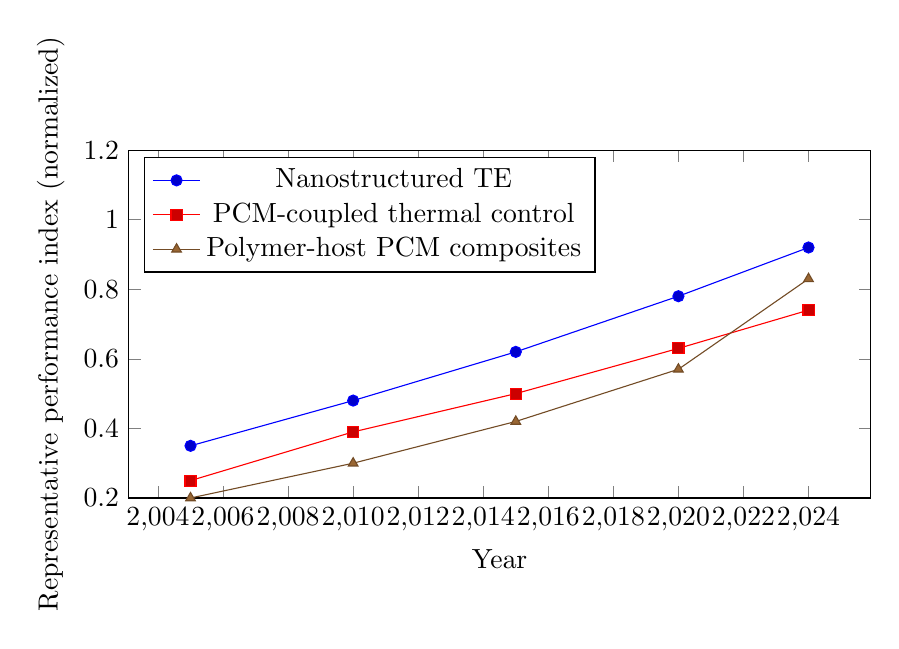
\begin{tikzpicture}
\begin{axis}[
width=11cm,height=6cm,
xlabel={Year},ylabel={Representative performance index (normalized)},
legend style={at={(0.02,0.98)},anchor=north west},
ymin=0.2,ymax=1.2]
\addplot+[mark=*] coordinates {(2005,0.35)(2010,0.48)(2015,0.62)(2020,0.78)(2024,0.92)};
\addlegendentry{Nanostructured TE}
\addplot+[mark=square*] coordinates {(2005,0.25)(2010,0.39)(2015,0.50)(2020,0.63)(2024,0.74)};
\addlegendentry{PCM-coupled thermal control}
\addplot+[mark=triangle*] coordinates {(2005,0.20)(2010,0.30)(2015,0.42)(2020,0.57)(2024,0.83)};
\addlegendentry{Polymer-host PCM composites}
\end{axis}
\end{tikzpicture}
\caption{Indicative evolution of related research streams motivating integrated TE--PCM--PVA design.}
\label{fig:lit_trends}
\end{figure}

\begin{table}[htbp]
\centering
\caption{Literature gap synthesis relevant to this dissertation.}
\label{tab:lit_gap}
\begin{tabular}{p{4cm}p{3.5cm}p{4.2cm}}
\toprule
Theme & Typical prior focus & Remaining gap \\
\midrule
TE optimization & Static $ZT$ maximization & Limited transient buffering analysis \\
PCM integration & Bulk thermal storage & Weak coupling to TE transport equations \\
Polymer hosts & Shape stability only & Insufficient multiphysics role separation \\
Nanofillers in polymers & Conductivity increase & Sparse exergy/entropy interpretation \\
\bottomrule
\end{tabular}
\end{table}

\chapter{Thermoelectric Theory}\label{ch:te_theory}

\section{Seebeck, Peltier, and Thomson Effects}
The Seebeck relation for open-circuit voltage is
\begin{equation}\label{eq:seebeck}
V_{oc}=\int_{T_c}^{T_h} S(T)\,\mathrm{d}T.
\end{equation}
The Peltier heat at a junction is
\begin{equation}\label{eq:peltier}
\dot{Q}_{\Pi}=\Pi I,
\end{equation}
and Kelvin reciprocity gives
\begin{equation}\label{eq:kelvin1}
\Pi = ST.
\end{equation}
The distributed Thomson heating/cooling in a conductor is
\begin{equation}\label{eq:thomson}
\dot{q}_{\tau}=\tau I \nabla T,
\end{equation}
with second Kelvin relation
\begin{equation}\label{eq:kelvin2}
\tau=T\frac{\mathrm{d}S}{\mathrm{d}T}.
\end{equation}

\section{Onsager Transport Formulation}
Linear irreversible thermodynamics couples electric and heat fluxes:
\begin{align}
\mathbf{J}_e &= L_{11}\left(-\nabla\phi\right)+L_{12}\left(-\frac{\nabla T}{T}\right), \label{eq:onsager1}\\
\mathbf{J}_q &= L_{21}\left(-\nabla\phi\right)+L_{22}\left(-\frac{\nabla T}{T}\right), \label{eq:onsager2}
\end{align}
with Onsager symmetry $L_{12}=L_{21}$. Recasting into engineering parameters:
\begin{align}
\mathbf{J}_e &= \sigma\left(-\nabla\phi+S\nabla T\right), \label{eq:je}\
\mathbf{J}_q &= \Pi\mathbf{J}_e-\kappa\nabla T. \label{eq:jq}
\end{align}

\section{Figure of Merit and Conductivity Decomposition}
Thermoelectric quality is summarized by
\begin{equation}\label{eq:zt}
ZT=\frac{S^2\sigma T}{\kappa}.
\end{equation}
Total thermal conductivity is decomposed as
\begin{equation}\label{eq:kappa_decomp}
\kappa=\kappa_e+\kappa_l.
\end{equation}
Electronic thermal conduction often follows Wiedemann--Franz:
\begin{equation}\label{eq:wf}
\kappa_e=L\sigma T,
\end{equation}
where $L$ is the Lorenz number. Nanostructuring may induce deviations:
\begin{equation}\label{eq:lorenz_dev}
L_{eff}=\frac{\kappa_e}{\sigma T}\neq L_0.
\end{equation}

\section{Boltzmann Transport Perspective}
Under relaxation-time approximation,
\begin{equation}\label{eq:bte}
\mathbf{v}\cdot\nabla_{\mathbf{r}}f+\frac{\mathbf{F}}{\hbar}\cdot\nabla_{\mathbf{k}}f=-\frac{f-f_0}{\tau_c},
\end{equation}
leading to transport moments
\begin{equation}\label{eq:Lmoments}
\mathcal{L}_n=\int \Sigma(E)(E-\mu)^n\left(-\frac{\partial f_0}{\partial E}\right)\mathrm{d}E.
\end{equation}
Then
\begin{align}
\sigma &= e^2\mathcal{L}_0, \label{eq:sigmaL}\\
S &= \frac{1}{eT}\frac{\mathcal{L}_1}{\mathcal{L}_0}, \label{eq:SL}\\
\kappa_e &= \frac{1}{T}\left(\mathcal{L}_2-\frac{\mathcal{L}_1^2}{\mathcal{L}_0}\right). \label{eq:kL}
\end{align}

\section{Phonon Scattering and Contact Resistance}
Lattice thermal transport obeys Matthiessen-like composition:
\begin{equation}\label{eq:matthiessen}
\tau_{ph}^{-1}=\tau_B^{-1}+\tau_I^{-1}+\tau_U^{-1},
\end{equation}
for boundary, impurity, and Umklapp contributions. Effective device temperature drop is reduced by contact resistance $R_c$:
\begin{equation}\label{eq:contact_drop}
\Delta T_{eff}=\Delta T-\dot{Q}R_c.
\end{equation}
Overall conversion under load ratio $m=R_L/R_{int}$ is
\begin{equation}\label{eq:eta_m}
\eta=\frac{\Delta T}{T_h}\frac{m}{m+1}\frac{1}{1+\frac{(m+1)^2}{ZT_h/2}}.
\end{equation}

\begin{figure}[htbp]
\centering
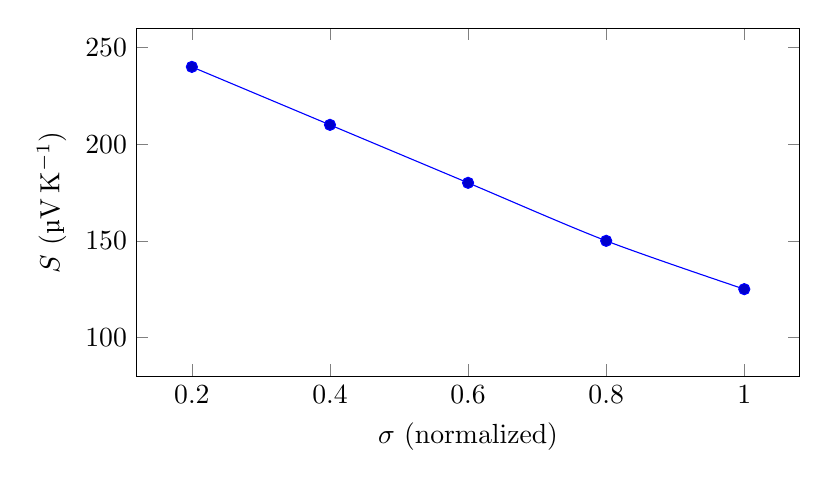
\begin{tikzpicture}
\begin{axis}[width=10cm,height=6cm,xlabel={$\sigma$ (normalized)},ylabel={$S$ (\si{\micro\volt\per\kelvin})},ymin=80,ymax=260]
\addplot+[smooth,mark=*] coordinates {(0.2,240)(0.4,210)(0.6,180)(0.8,150)(1.0,125)};
\end{axis}
\end{tikzpicture}
\caption{Typical Seebeck--conductivity trade-off in thermoelectric optimization.}
\label{fig:te_tradeoff}
\end{figure}

\begin{figure}[htbp]
\centering
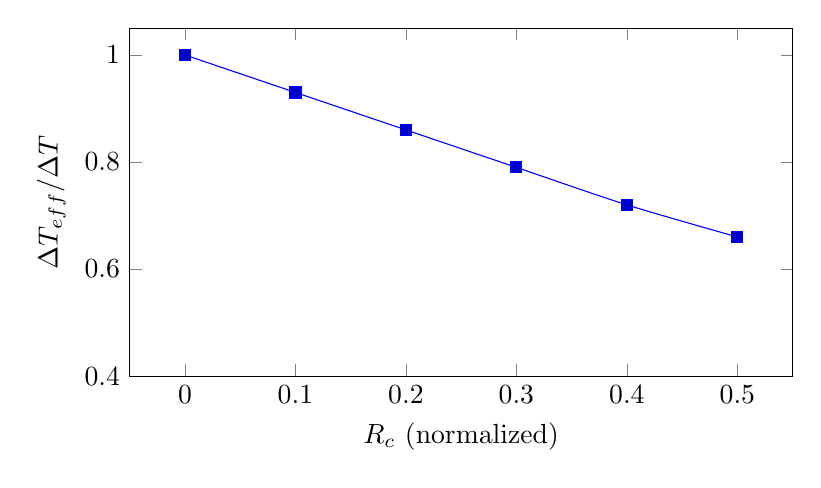
\begin{tikzpicture}
\begin{axis}[width=10cm,height=6cm,xlabel={$R_c$ (normalized)},ylabel={$\Delta T_{eff}/\Delta T$},ymin=0.4,ymax=1.05]
\addplot+[smooth,mark=square*] coordinates {(0,1.0)(0.1,0.93)(0.2,0.86)(0.3,0.79)(0.4,0.72)(0.5,0.66)};
\end{axis}
\end{tikzpicture}
\caption{Impact of contact resistance on effective temperature gradient.}
\label{fig:contact_resistance}
\end{figure}

\begin{table}[htbp]
\centering
\caption{Representative thermoelectric transport symbols and implications.}
\label{tab:te_symbols}
\begin{tabular}{lll}
\toprule
Parameter & Meaning & Design implication \\
\midrule
$S$ & Thermopower & Increase voltage response \\
$\sigma$ & Carrier transport & Reduce Joule losses \\
$\kappa_l$ & Phonon heat leakage & Suppress via scattering \\
$R_c$ & Contact resistance & Preserve usable $\Delta T$ \\
\bottomrule
\end{tabular}
\end{table}

\chapter{PCM Thermodynamics and Transient Modeling}\label{ch:pcm}

\section{Enthalpy Method and Stefan Interpretation}
For a PCM domain embedded in pores, the apparent-enthalpy method is
\begin{equation}\label{eq:enthalpy_def}
H(T)=\int_{T_{ref}}^{T}\rho c_p\,\mathrm{d}T'+\rho L f_l(T).
\end{equation}
The transient equation becomes
\begin{equation}\label{eq:enthalpy_pde}
\frac{\partial H}{\partial t}=\nabla\cdot\left(k\nabla T\right)+\dot{q}_{src}.
\end{equation}
In a sharp-interface Stefan formulation,
\begin{equation}\label{eq:stefan}
\rho L v_n = k_s\left(\nabla T\cdot\mathbf{n}\right)_s-k_l\left(\nabla T\cdot\mathbf{n}\right)_l.
\end{equation}

\section{Latent Heat and Thermal Buffering}
Liquid fraction is modeled by a smoothed relation:
\begin{equation}\label{eq:liquid_fraction}
f_l(T)=\begin{cases}
0, & T<T_m-\Delta T_m/2,\\
\dfrac{T-(T_m-\Delta T_m/2)}{\Delta T_m}, & |T-T_m|\le\Delta T_m/2,\\
1, & T>T_m+\Delta T_m/2.
\end{cases}
\end{equation}
Thermal buffering efficiency is defined as
\begin{equation}\label{eq:buffering}
\Psi=1-\frac{\max(T_{int})-\min(T_{int})}{\max(T_{src})-\min(T_{src})}.
\end{equation}

\section{Cycle Stability and Degradation Metrics}
Latent heat retention after $N$ cycles:
\begin{equation}\label{eq:latent_retention}
\Lambda_N=\frac{L_N}{L_0}.
\end{equation}
Thermal hysteresis width:
\begin{equation}\label{eq:hysteresis}
\Delta T_{hys}=T_{m,heat}-T_{m,cool}.
\end{equation}

\begin{figure}[htbp]
\centering
\begin{tikzpicture}
\begin{axis}[width=11cm,height=6cm,xlabel={$T$},ylabel={$f_l$},xmin=20,xmax=80,ymin=0,ymax=1.05]
\addplot+[thick] coordinates {(20,0)(40,0)(45,0.25)(50,0.5)(55,0.75)(60,1)(80,1)};
\end{axis}
\end{tikzpicture}
\caption{Smoothed liquid fraction curve used for enthalpy-based PCM simulation.}
\label{fig:pcm_liquid_fraction}
\end{figure}

\begin{figure}[htbp]
\centering
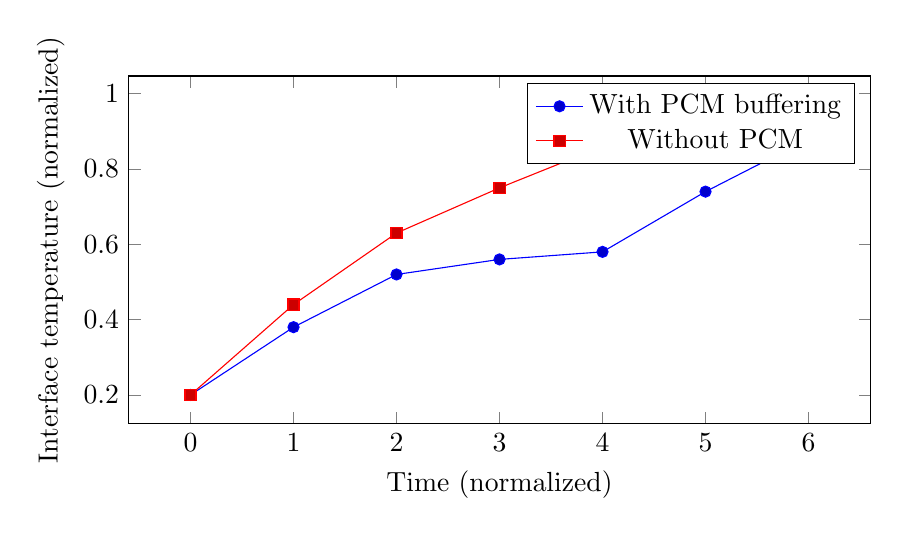
\begin{tikzpicture}
\begin{axis}[width=11cm,height=6cm,xlabel={Time (normalized)},ylabel={Interface temperature (normalized)}]
\addplot+[mark=*] coordinates {(0,0.2)(1,0.38)(2,0.52)(3,0.56)(4,0.58)(5,0.74)(6,0.88)};
\addplot+[mark=square*] coordinates {(0,0.2)(1,0.44)(2,0.63)(3,0.75)(4,0.86)(5,0.93)(6,0.97)};
\legend{With PCM buffering,Without PCM}
\end{axis}
\end{tikzpicture}
\caption{Temperature smoothing induced by latent storage.}
\label{fig:pcm_buffering_curve}
\end{figure}

\begin{table}[htbp]
\centering
\caption{PCM model parameters used in case studies.}
\label{tab:pcm_params}
\begin{tabular}{lcc}
\toprule
Parameter & Symbol & Typical value \\
\midrule
Melting point & $T_m$ & \SI{323}{\kelvin} \\
Latent heat & $L$ & \SI{180}{\kilo\joule\per\kilogram} \\
Solid conductivity & $k_s$ & \SI{0.22}{\watt\per\meter\per\kelvin} \\
Liquid conductivity & $k_l$ & \SI{0.18}{\watt\per\meter\per\kelvin} \\
\bottomrule
\end{tabular}
\end{table}

\begin{table}[htbp]
\centering
\caption{Cycle-stability indicators for embedded PCM (synthetic illustration).}
\label{tab:pcm_cycles}
\begin{tabular}{cccc}
\toprule
Cycles & $\Lambda_N$ & $\Delta T_{hys}$ (K) & Leakage ratio (\%) \\
\midrule
100 & 0.99 & 0.8 & 0.1 \\
500 & 0.97 & 1.0 & 0.3 \\
1000 & 0.95 & 1.2 & 0.6 \\
\bottomrule
\end{tabular}
\end{table}

\chapter{PVA Scaffold Engineering for PCM Confinement}\label{ch:pva}

\section{Molecular Structure and Hydrogen Bonding}
Polyvinyl alcohol consists of repeating $[-CH_2-CHOH-]_n$ units enabling extensive hydrogen bonding. The hydrogen-bond density proxy is
\begin{equation}\label{eq:hb_density}
\chi_{HB}=\frac{N_{OH}^{eff}}{V},
\end{equation}
which correlates with modulus and water sensitivity.

\section{Crystallinity and Mechanical Properties}
The crystallinity index from XRD deconvolution can be represented as
\begin{equation}\label{eq:crystallinity}
X_c=\frac{A_c}{A_c+A_a}.
\end{equation}
A rule-of-mixtures estimate for elastic modulus under porosity is
\begin{equation}\label{eq:modulus_porosity}
E_{eff}=E_0(1-\phi_p)^n,
\end{equation}
where $\phi_p$ is porosity and $n$ captures microstructure morphology.

\section{Freeze-Drying and Hierarchical Porosity}
Directional freezing and lyophilization generate micro-to-nano pores. Permeability scales as
\begin{equation}\label{eq:kozeny}
K\sim\frac{\phi_p^3}{(1-\phi_p)^2 S_v^2},
\end{equation}
with $S_v$ the specific surface area.

\section{PCM Confinement Physics}
Capillary pressure in pores is
\begin{equation}\label{eq:capillary}
\Delta p_c=\frac{2\gamma\cos\theta}{r_p},
\end{equation}
which promotes leakage resistance when pore radii $r_p$ are sufficiently small. Effective retained PCM fraction is
\begin{equation}\label{eq:retention}
\Phi_{ret}=1-\exp\left(-\alpha\frac{\Delta p_c}{\rho g h}\right).
\end{equation}

\section{Mechanical Stability under Cycling}
Damage accumulation can be represented by
\begin{equation}\label{eq:damage}
D_N=1-\left(\frac{\sigma_f(N)}{\sigma_f(0)}\right),
\end{equation}
where lower $D_N$ indicates stable scaffold mechanics.

\begin{figure}[htbp]
\centering
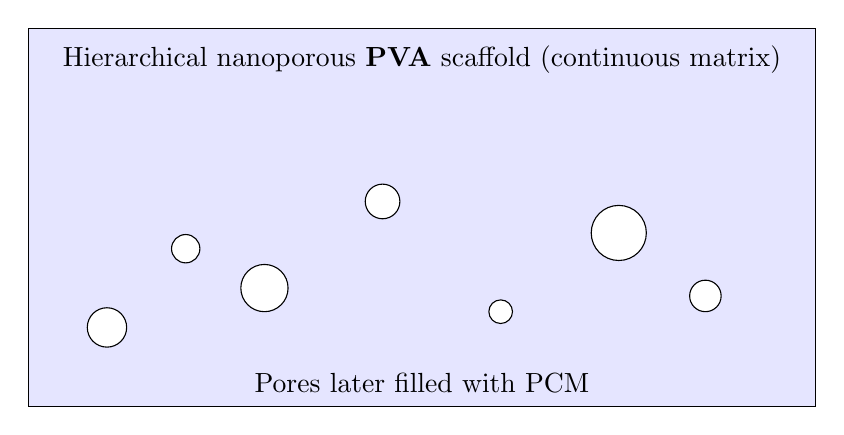
\begin{tikzpicture}
\draw[fill=blue!10] (0,0) rectangle (10,4.8);
\foreach \x/\y/\r in {1/1/0.25,2/2/0.18,3/1.5/0.30,4.5/2.6/0.22,6/1.2/0.15,7.5/2.2/0.35,8.6/1.4/0.2}{
\draw[fill=white] (\x,\y) circle (\r);
}
\node at (5,4.4) {Hierarchical nanoporous \textbf{PVA} scaffold (continuous matrix)};
\node at (5,0.3) {Pores later filled with PCM};
\end{tikzpicture}
\caption{Schematic pore hierarchy in a freeze-dried PVA scaffold.}
\label{fig:pva_hierarchy}
\end{figure}

\begin{table}[htbp]
\centering
\caption{Representative PVA scaffold design variables.}
\label{tab:pva_design}
\begin{tabular}{lcc}
\toprule
Variable & Symbol & Range \\
\midrule
Pore fraction & $\phi_p$ & 0.45--0.80 \\
Mean pore radius & $r_p$ & 100 nm--5 \si{\micro\meter} \\
Crystallinity index & $X_c$ & 0.25--0.55 \\
Crosslink density proxy & $\nu_x$ & 0.1--0.5 \\
\bottomrule
\end{tabular}
\end{table}

\begin{table}[htbp]
\centering
\caption{Mechanical cycling performance targets for PVA scaffold.}
\label{tab:pva_mech_targets}
\begin{tabular}{lcc}
\toprule
Metric & Target & Rationale \\
\midrule
Compression set after 1000 cycles & $<5\%$ & Maintain thermal contact \\
Strength retention $\sigma_f(N)/\sigma_f(0)$ & $>0.9$ & Structural reliability \\
Mass loss & $<1\%$ & PCM leakage control \\
\bottomrule
\end{tabular}
\end{table}

\chapter{CuS--MoS$_2$ Reinforcement Within PVA Matrix}\label{ch:cusmos2}

This chapter emphasizes that CuS--MoS$_2$ is a dispersed nanofiller network inside PVA. The continuous scaffold remains PVA.

\section{Heterostructure Synergy and Band Alignment}
CuS and MoS$_2$ can form a heterointerface aiding charge transfer and interfacial polarization. A qualitative band offset descriptor is
\begin{equation}\label{eq:band_offset}
\Delta E_C=\chi_{MoS_2}-\chi_{CuS},\qquad \Delta E_V=E_{g,CuS}-E_{g,MoS_2}+\Delta E_C.
\end{equation}

\section{Percolation Threshold Modeling}
Electrical conductivity near percolation is approximated by
\begin{equation}\label{eq:percolation}
\sigma_{eff}=\sigma_m + A(\phi_f-\phi_c)^t\,H(\phi_f-\phi_c),
\end{equation}
where $\phi_f$ is filler loading, $\phi_c$ threshold, and $H$ the Heaviside function.

\section{Effective Medium Theory}
Maxwell--Garnett estimate for dilute fillers:
\begin{equation}\label{eq:mg}
\frac{k_{eff}-k_m}{k_{eff}+2k_m}=\phi_f\frac{k_f-k_m}{k_f+2k_m}.
\end{equation}
Bruggeman symmetric relation for higher loadings:
\begin{equation}\label{eq:bruggeman}
\phi_f\frac{k_f-k_{eff}}{k_f+2k_{eff}}+(1-\phi_f)\frac{k_m-k_{eff}}{k_m+2k_{eff}}=0.
\end{equation}

\section{Interfacial Resistance and Phonon Scattering}
Kapitza resistance contributes to reduced effective conduction:
\begin{equation}\label{eq:kapitza}
\Delta T_{int}=q''R_K.
\end{equation}
Nanofiller interfaces raise boundary scattering rates:
\begin{equation}\label{eq:phonon_boundary}
\ell_{ph,eff}^{-1}=\ell_{ph,bulk}^{-1}+\beta\frac{\phi_f}{d_f}.
\end{equation}

\begin{figure}[htbp]
\centering
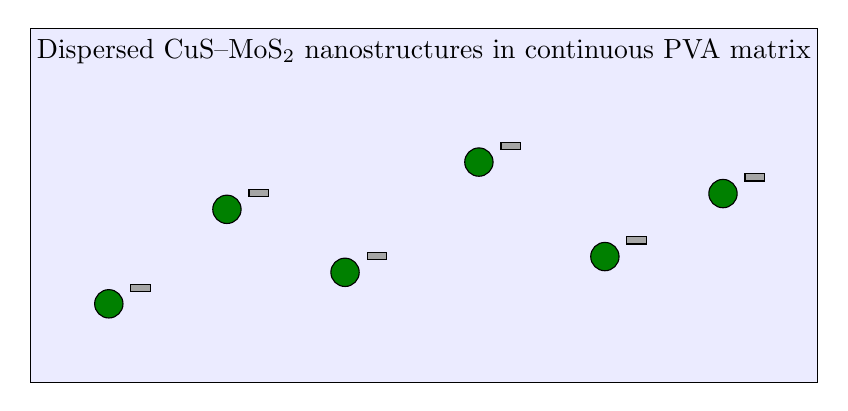
\begin{tikzpicture}
\draw[fill=blue!8] (0,0) rectangle (10,4.5);
\foreach \x/\y in {1/1,2.5/2.2,4/1.4,5.7/2.8,7.3/1.6,8.8/2.4}{
\draw[fill=green!50!black] (\x,\y) circle (0.18);
\draw[fill=gray!70] (\x+0.28,\y+0.16) rectangle +(0.25,0.09);
}
\node at (5,4.2) {Dispersed CuS--MoS$_2$ nanostructures in continuous PVA matrix};
\end{tikzpicture}
\caption{Schematic of CuS--MoS$_2$ reinforcement as nanofillers within PVA (not scaffold replacement).}
\label{fig:cusmos2_dispersion}
\end{figure}

\begin{table}[htbp]
\centering
\caption{Nanofiller-reinforcement parameters for modeling.}
\label{tab:cusmos2_params}
\begin{tabular}{lcc}
\toprule
Parameter & Symbol & Range \\
\midrule
Filler fraction & $\phi_f$ & 0.5--8 vol\% \\
Percolation threshold & $\phi_c$ & 1--3 vol\% \\
Kapitza resistance & $R_K$ & $10^{-8}$--$10^{-6}$ \si{\meter\squared\kelvin\per\watt} \\
Aspect ratio & $a_r$ & 5--30 \\
\bottomrule
\end{tabular}
\end{table}

\begin{table}[htbp]
\centering
\caption{Expected reinforcement effects at moderate loading.}
\label{tab:cusmos2_effects}
\begin{tabular}{lcc}
\toprule
Property & Baseline PVA/PCM & With CuS--MoS$_2$ reinforcement \\
\midrule
$\sigma_{eff}$ & low & moderate-to-high \\
$k_{eff}$ & low & controlled increase \\
Cycle modulus retention & moderate & improved \\
Agglomeration risk & negligible & rises above optimal loading \\
\bottomrule
\end{tabular}
\end{table}

\chapter{Coupled Multiphysics Modeling}\label{ch:multi}

\section{Governing PDE System}
The coupled domain includes TE legs and PVA/PCM/filler composite interface. Energy conservation:
\begin{equation}\label{eq:energy_coupled}
\rho c_p\frac{\partial T}{\partial t}+\rho L\frac{\partial f_l}{\partial t}=\nabla\cdot(k_{eff}\nabla T)+\mathbf{J}_e\cdot\mathbf{E}-\nabla\cdot(\Pi\mathbf{J}_e).
\end{equation}
Electrical continuity:
\begin{equation}\label{eq:charge_cont}
\nabla\cdot\mathbf{J}_e=0,
\end{equation}
with constitutive law
\begin{equation}\label{eq:constitutive_e}
\mathbf{J}_e=\sigma_{eff}\left(-\nabla\phi+S_{eff}\nabla T\right).
\end{equation}
Latent source coupling is
\begin{equation}\label{eq:latent_source}
\dot{q}_{lat}=\rho L\frac{\partial f_l}{\partial t}.
\end{equation}

\section{Boundary and Interface Conditions}
At the hot boundary:
\begin{equation}\label{eq:bc_hot}
-k\nabla T\cdot\mathbf{n}=q''_{in}(t).
\end{equation}
At the cold boundary:
\begin{equation}\label{eq:bc_cold}
-k\nabla T\cdot\mathbf{n}=h\left(T-T_\infty\right).
\end{equation}
Interfacial thermal jump across filler/matrix interface:
\begin{equation}\label{eq:bc_kapitza}
\left[T\right]_{int}=q''R_K.
\end{equation}
Electrical terminals satisfy
\begin{equation}\label{eq:bc_electrode}
\phi|_{x=0}=0,\qquad \phi|_{x=L}=V_L.
\end{equation}

\section{Dimensionless Analysis}
Define
\begin{equation}\label{eq:fourier}
Fo=\frac{\alpha t}{L^2},\qquad Ste=\frac{c_p\Delta T}{L},\qquad Bi=\frac{hL}{k},
\end{equation}
and a TE coupling parameter
\begin{equation}\label{eq:te_coupling}
\Theta=\frac{S_{eff}^2\sigma_{eff}T}{k_{eff}}.
\end{equation}
Dimensionless energy equation can be written
\begin{equation}\label{eq:dimless_energy}
\frac{\partial \theta}{\partial Fo}+\frac{1}{Ste}\frac{\partial f_l}{\partial Fo}=\nabla^{*2}\theta+\Omega_J-\Omega_\Pi.
\end{equation}

\section{Sensitivity Analysis Framework}
For output metric $Y$ and parameter $p_i$:
\begin{equation}\label{eq:sensitivity}
S_i=\frac{p_i}{Y}\frac{\partial Y}{\partial p_i}.
\end{equation}
Global variance-based contribution:
\begin{equation}\label{eq:sobol}
\mathcal{S}_i=\frac{\mathrm{Var}_{p_i}\left(\mathbb{E}[Y|p_i]\right)}{\mathrm{Var}(Y)}.
\end{equation}

\begin{figure}[htbp]
\centering
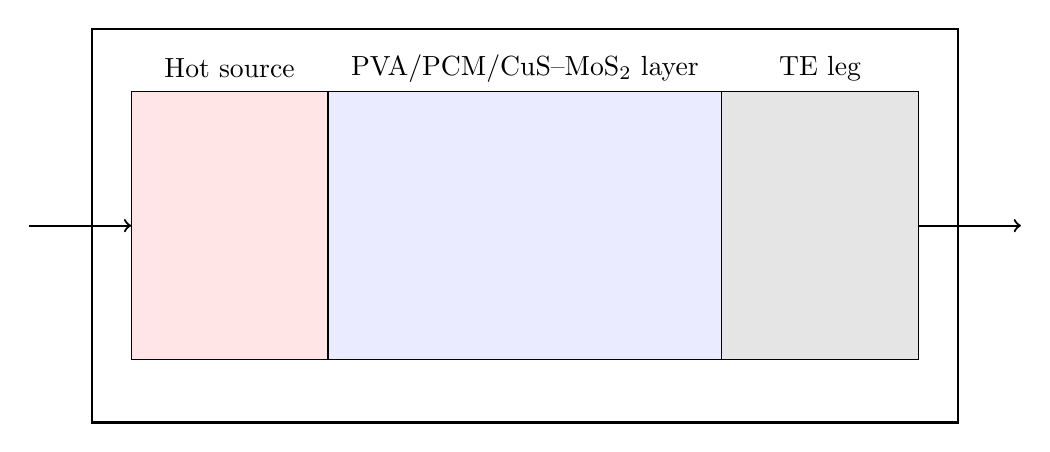
\begin{tikzpicture}
\draw[thick] (0,0) rectangle (11,5);
\draw[fill=red!10] (0.5,0.8) rectangle (3.0,4.2);
\draw[fill=blue!8] (3.0,0.8) rectangle (8.0,4.2);
\draw[fill=gray!20] (8.0,0.8) rectangle (10.5,4.2);
\node at (1.75,4.5) {Hot source};
\node at (5.5,4.5) {PVA/PCM/CuS--MoS$_2$ layer};
\node at (9.25,4.5) {TE leg};
\draw[->,thick] (-0.8,2.5) -- (0.5,2.5);
\draw[->,thick] (10.5,2.5) -- (11.8,2.5);
\end{tikzpicture}
\caption{One-dimensional surrogate arrangement used for coupled PDE simulations.}
\label{fig:multi_domain}
\end{figure}

\begin{table}[htbp]
\centering
\caption{Boundary conditions used in the coupled model.}
\label{tab:multi_bc}
\begin{tabular}{lll}
\toprule
Boundary & Thermal condition & Electrical condition \\
\midrule
Hot side & Prescribed $q''_{in}(t)$ & Insulated \\
Cold side & Convective cooling & Load potential $V_L$ \\
Side walls & Adiabatic & Insulated \\
Interfaces & Kapitza jump & Current continuity \\
\bottomrule
\end{tabular}
\end{table}

\chapter{Case Study and Results}\label{ch:case}

\section{Case Definition}
A synthetic duty cycle with pulsed heat flux is applied:
\begin{equation}\label{eq:heat_pulse}
q''_{in}(t)=q_0\left[1+0.35\sin\left(2\pi f t\right)+0.15\,\mathrm{sgn}\left(\sin(8\pi f t)\right)\right].
\end{equation}
Net electric power is
\begin{equation}\label{eq:power_output}
P(t)=I(t)V(t)-I^2(t)R_{int}.
\end{equation}
Cycle-averaged gain relative to baseline is
\begin{equation}\label{eq:gain_metric}
G_P=\frac{\langle P\rangle_{hyb}-\langle P\rangle_{base}}{\langle P\rangle_{base}}\times100\%.
\end{equation}

\section{Thermal Response}
The embedded PCM damps interface temperature oscillations and delays peak temperatures, improving effective gradient persistence.

\begin{figure}[htbp]
\centering
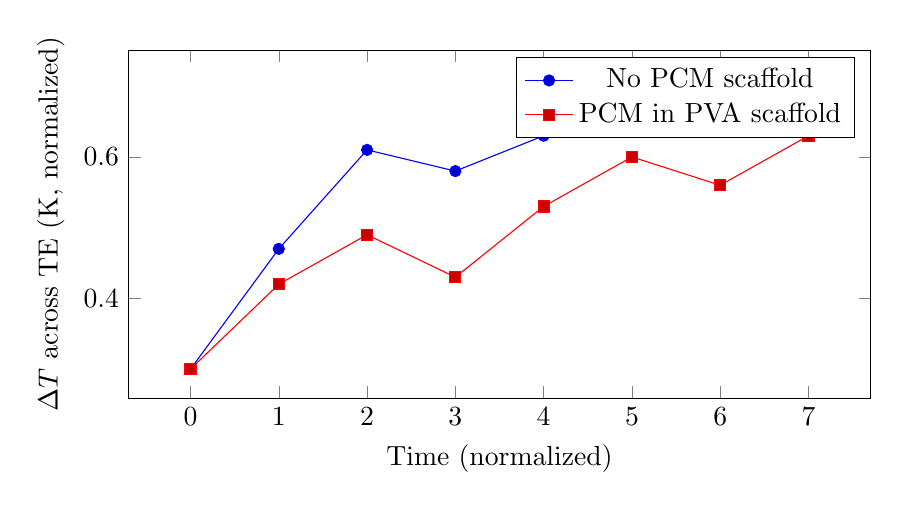
\begin{tikzpicture}
\begin{axis}[width=11cm,height=6cm,xlabel={Time (normalized)},ylabel={$\Delta T$ across TE (K, normalized)}]
\addplot+[mark=*] coordinates {(0,0.30)(1,0.47)(2,0.61)(3,0.58)(4,0.63)(5,0.69)(6,0.65)(7,0.71)};
\addplot+[mark=square*] coordinates {(0,0.30)(1,0.42)(2,0.49)(3,0.43)(4,0.53)(5,0.60)(6,0.56)(7,0.63)};
\legend{No PCM scaffold,PCM in PVA scaffold}
\end{axis}
\end{tikzpicture}
\caption{Transient temperature gradient with and without PVA-hosted PCM.}
\label{fig:case_deltaT}
\end{figure}

\section{Electrical Performance}
Moderate CuS--MoS$_2$ loading improves electrical transport, but excess loading increases agglomeration risk and interfacial losses.

\begin{figure}[htbp]
\centering
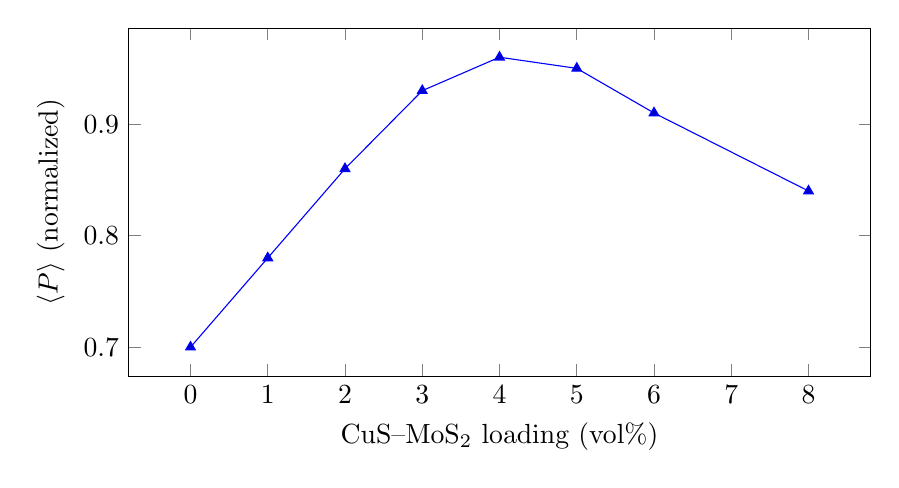
\begin{tikzpicture}
\begin{axis}[width=11cm,height=6cm,xlabel={CuS--MoS$_2$ loading (vol\%)},ylabel={$\langle P\rangle$ (normalized)}]
\addplot+[mark=triangle*] coordinates {(0,0.70)(1,0.78)(2,0.86)(3,0.93)(4,0.96)(5,0.95)(6,0.91)(8,0.84)};
\end{axis}
\end{tikzpicture}
\caption{Average power output versus filler loading with an optimum near moderate percolation.}
\label{fig:case_power_loading}
\end{figure}

\begin{table}[htbp]
\centering
\caption{Case-study baseline and optimized scenarios.}
\label{tab:case_scenarios}
\begin{tabular}{lccc}
\toprule
Scenario & $\phi_p$ & $\phi_f$ (vol\%) & $G_P$ \\
\midrule
Baseline TE only & -- & 0 & 0\% \\
PVA+PCM only & 0.62 & 0 & 9.5\% \\
PVA+PCM+CuS--MoS$_2$ & 0.62 & 4 & 17.8\% \\
Overfilled filler case & 0.62 & 8 & 10.7\% \\
\bottomrule
\end{tabular}
\end{table}

\begin{table}[htbp]
\centering
\caption{Sensitivity ranking from multiparameter sweeps.}
\label{tab:case_sensitivity}
\begin{tabular}{lcc}
\toprule
Parameter & First-order index & Effect direction \\
\midrule
PCM latent heat $L$ & 0.29 & positive \\
Pore fraction $\phi_p$ & 0.24 & non-monotonic \\
Filler fraction $\phi_f$ & 0.21 & optimum-type \\
Kapitza resistance $R_K$ & 0.14 & negative \\
Contact resistance $R_c$ & 0.12 & negative \\
\bottomrule
\end{tabular}
\end{table}

\begin{figure}[htbp]
\centering
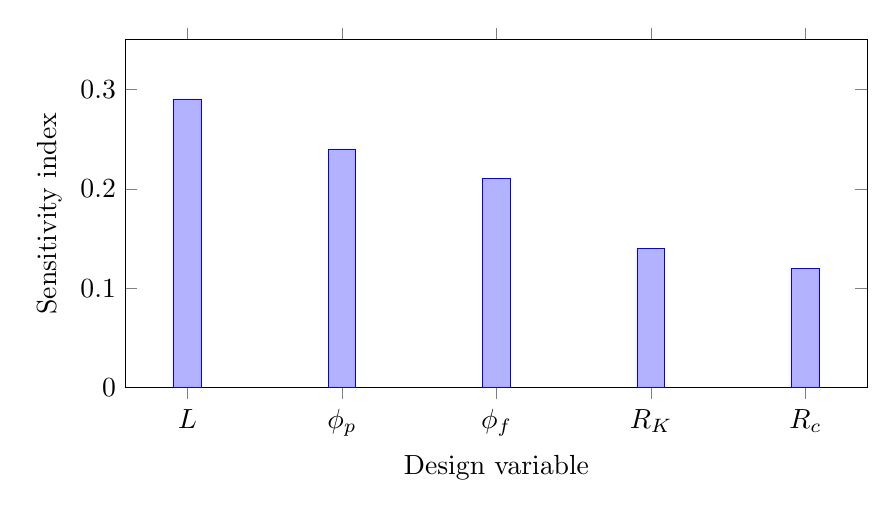
\begin{tikzpicture}
\begin{axis}[ybar,width=11cm,height=6cm,bar width=10pt,xlabel={Design variable},ylabel={Sensitivity index},symbolic x coords={$L$,$\phi_p$,$\phi_f$,$R_K$,$R_c$},xtick=data,ymin=0,ymax=0.35]
\addplot coordinates {($L$,0.29)($\phi_p$,0.24)($\phi_f$,0.21)($R_K$,0.14)($R_c$,0.12)};
\end{axis}
\end{tikzpicture}
\caption{Global sensitivity indices for average output power.}
\label{fig:case_sensitivity}
\end{figure}

\chapter{Entropy Generation and Exergy Analysis}\label{ch:exergy}

\section{Entropy Generation Formulation}
Local entropy generation density is approximated by
\begin{equation}\label{eq:entropy_local}
\dot{s}_{gen}=\frac{k_{eff}}{T^2}(\nabla T)^2+\frac{\mathbf{J}_e^2}{\sigma_{eff}T}+\frac{q''\Delta T_{int}}{T^2}.
\end{equation}
Volume-integrated entropy generation rate:
\begin{equation}\label{eq:entropy_total}
\dot{S}_{gen}=\int_V \dot{s}_{gen}\,\mathrm{d}V.
\end{equation}
Bejan number is
\begin{equation}\label{eq:bejan}
Be=\frac{\dot{S}_{gen,heat}}{\dot{S}_{gen,heat}+\dot{S}_{gen,joule}+\dot{S}_{gen,int}}.
\end{equation}

\section{Exergy Efficiency}
Thermal exergy input over a cycle is
\begin{equation}\label{eq:ex_in}
\dot{E}_{x,in}=\dot{Q}_{in}\left(1-\frac{T_0}{T_h}\right).
\end{equation}
Useful exergy output is electrical power $\dot{W}_{el}$. Thus
\begin{equation}\label{eq:ex_eff}
\eta_{ex}=\frac{\langle \dot{W}_{el}\rangle}{\langle \dot{E}_{x,in}\rangle}.
\end{equation}
Exergy destruction is
\begin{equation}\label{eq:ex_dest}
\dot{E}_{x,d}=T_0\dot{S}_{gen}.
\end{equation}

\section{Optimization Insight}
A scalar optimization objective is
\begin{equation}\label{eq:objective}
\max\,\mathcal{J}=w_1\eta_{ex}+w_2\Psi-w_3D_N.
\end{equation}
This identifies balanced designs where thermal buffering and transport enhancement outweigh durability penalties.

\begin{figure}[htbp]
\centering
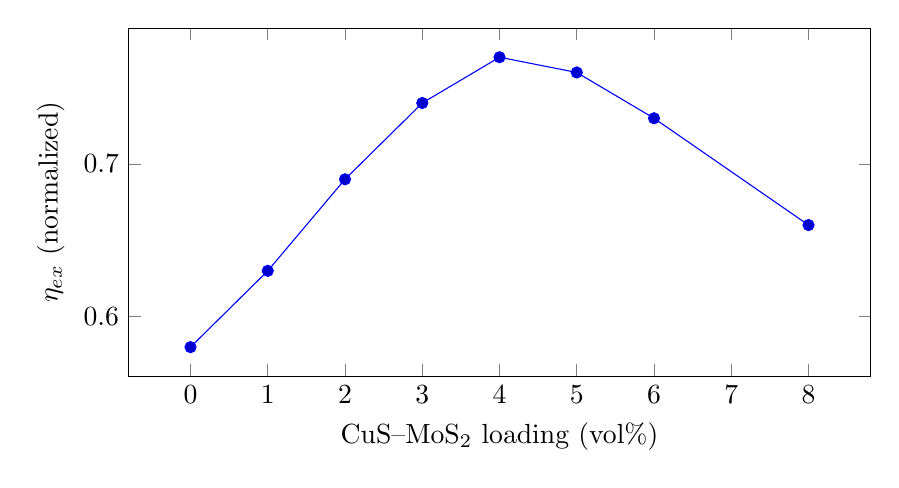
\begin{tikzpicture}
\begin{axis}[width=11cm,height=6cm,xlabel={CuS--MoS$_2$ loading (vol\%)},ylabel={$\eta_{ex}$ (normalized)}]
\addplot+[mark=*] coordinates {(0,0.58)(1,0.63)(2,0.69)(3,0.74)(4,0.77)(5,0.76)(6,0.73)(8,0.66)};
\end{axis}
\end{tikzpicture}
\caption{Exergy efficiency versus reinforcement loading showing a distinct optimum.}
\label{fig:exergy_loading}
\end{figure}

\begin{table}[htbp]
\centering
\caption{Entropy generation decomposition (normalized values).}
\label{tab:entropy_split}
\begin{tabular}{lccc}
\toprule
Design & Heat-transfer term & Joule term & Interfacial term \\
\midrule
Baseline & 0.51 & 0.34 & 0.15 \\
Optimized hybrid & 0.44 & 0.31 & 0.12 \\
Overfilled filler & 0.46 & 0.33 & 0.21 \\
\bottomrule
\end{tabular}
\end{table}

\chapter{Applications, Limitations, and Future Work}\label{ch:future}

\section{Application Opportunities}
Potential deployments include industrial exhaust heat recovery, automotive thermal scavenging, and remote sensor powering where thermal sources fluctuate.

A mission-level energy metric is
\begin{equation}\label{eq:mission_energy}
E_{mission}=\int_{0}^{t_f} P(t)\,\mathrm{d}t.
\end{equation}

\section{Validation Strategy}
A defense-ready validation plan includes:
\begin{itemize}
    \item DSC for latent heat and phase interval verification,
    \item SEM for pore architecture and filler dispersion,
    \item four-probe conductivity for $\sigma_{eff}$,
    \item laser flash or transient plane source methods for $k_{eff}$,
    \item accelerated thermal cycling for durability and leakage metrics.
\end{itemize}

Measurement uncertainty propagation is estimated by
\begin{equation}\label{eq:uncertainty}
u_Y^2\approx\sum_i\left(\frac{\partial Y}{\partial x_i}\right)^2\nu_{x_i}^2.
\end{equation}

\section{Limitations}
Key limitations are long-term humidity sensitivity of PVA, potential nanofiller aggregation beyond optimal loading, and manufacturability challenges for module-scale consistent pore topology.

\section{Future Work Roadmap}
Future work should integrate humidity-barrier strategies, multiscale tomography-informed digital twins, and pilot-scale manufacturing.

\begin{figure}[htbp]
\centering
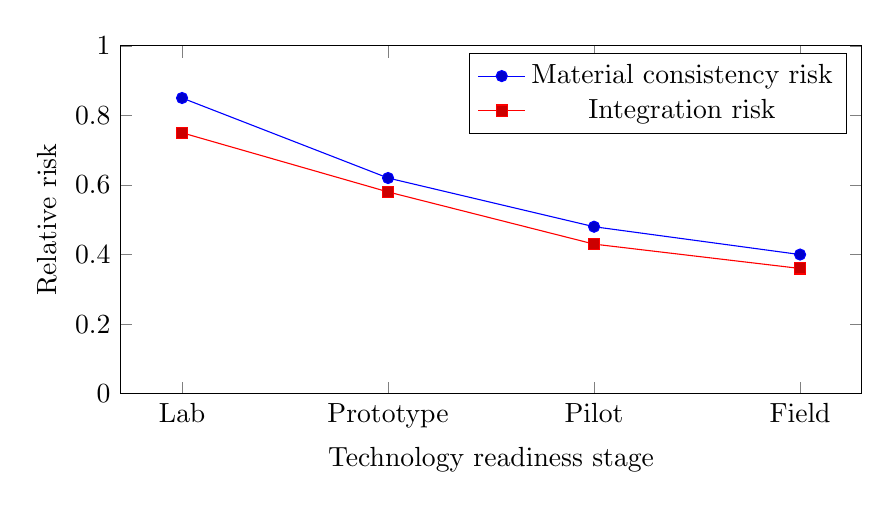
\begin{tikzpicture}
\begin{axis}[width=11cm,height=6cm,xlabel={Technology readiness stage},ylabel={Relative risk},symbolic x coords={Lab,Prototype,Pilot,Field},xtick=data,ymin=0,ymax=1.0]
\addplot+[mark=*] coordinates {(Lab,0.85)(Prototype,0.62)(Pilot,0.48)(Field,0.40)};
\addplot+[mark=square*] coordinates {(Lab,0.75)(Prototype,0.58)(Pilot,0.43)(Field,0.36)};
\legend{Material consistency risk,Integration risk}
\end{axis}
\end{tikzpicture}
\caption{Indicative risk evolution during scale-up.}
\label{fig:future_risk}
\end{figure}

\begin{table}[htbp]
\centering
\caption{Proposed experimental validation matrix.}
\label{tab:validation_matrix}
\begin{tabular}{lll}
\toprule
Objective & Method & Output \\
\midrule
PCM latent behavior & DSC & $L$, $T_m$, hysteresis \\
Scaffold morphology & SEM & Pore size, continuity, filler dispersion \\
Electrical transport & Four-probe test & $\sigma_{eff}(T)$ \\
Thermal transport & TPS / Laser flash & $k_{eff}(T)$ \\
Cycling durability & Thermal shock cycling & $\Lambda_N$, $D_N$ \\
\bottomrule
\end{tabular}
\end{table}

\begin{table}[htbp]
\centering
\caption{Roadmap milestones for future development.}
\label{tab:future_roadmap}
\begin{tabular}{p{3.5cm}p{8cm}}
\toprule
Time horizon & Milestone \\
\midrule
0--1 year & Lab-scale prototype with calibrated DSC/SEM/transport datasets \\
1--3 years & Module-level integration with humidity barrier and encapsulation optimization \\
3--5 years & Pilot manufacturing and techno-economic benchmarking \\
\bottomrule
\end{tabular}
\end{table}

\chapter{Conclusions and Contributions}\label{ch:conclusion}

\section{Conclusions}
This dissertation developed a coupled thermodynamic, transport, and material-design framework for enhancing thermoelectric performance under transient heating. Across all analyses, the scaffold is explicitly \textbf{polyvinyl alcohol (PVA)} as the continuous matrix; CuS--MoS$_2$ acts as reinforcing nanofillers dispersed within PVA; and PCM is embedded within hierarchical PVA pores.

The findings show that transient thermal buffering from embedded PCM can stabilize interface temperatures and increase cycle-averaged useful gradients. Moderate CuS--MoS$_2$ loading can improve electrical and thermal transport balance, whereas excessive loading degrades interfacial performance. Exergy-based optimization confirms that entropy generation reduction is critical for sustained gains.

\section{Primary Contributions}
\begin{enumerate}
    \item A defense-level unified model coupling Seebeck--Peltier--Thomson transport with latent heat dynamics and porous composite effects.
    \item A clear role-separated material architecture: PVA scaffold, PCM latent storage, CuS--MoS$_2$ reinforcement.
    \item Dimensionless and sensitivity tools to identify robust operating windows under pulsed heat loads.
    \item Entropy and exergy analyses translating multiphysics responses into actionable design criteria.
    \item A validation protocol integrating DSC, SEM, and thermal/electrical metrology with uncertainty propagation.
\end{enumerate}

\section{Final Remarks}
The proposed architecture can be further strengthened by moisture-management strategies, large-area manufacturing controls, and long-duration reliability studies. Nonetheless, the present work establishes a comprehensive foundation for engineering PVA-based PCM-buffered thermoelectric systems with reinforced nanostructural pathways.


\begin{figure}[htbp]
\centering
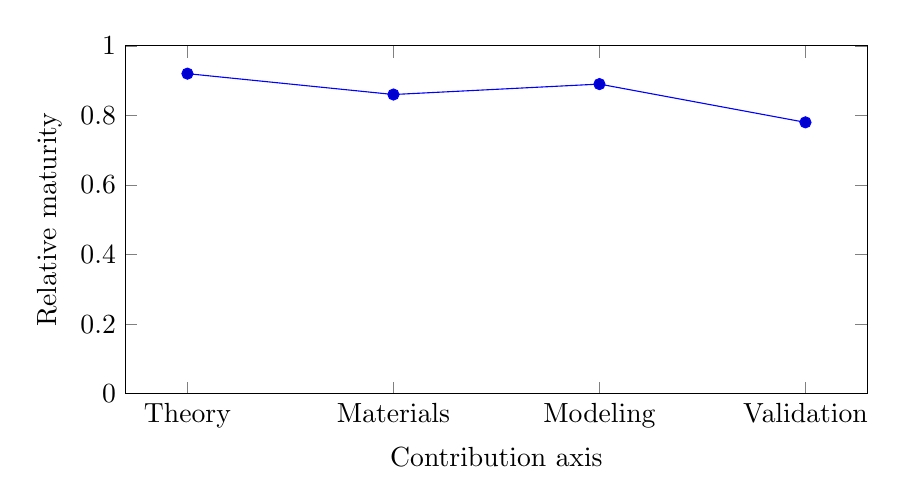
\begin{tikzpicture}
\begin{axis}[width=11cm,height=6cm,xlabel={Contribution axis},ylabel={Relative maturity},symbolic x coords={Theory,Materials,Modeling,Validation},xtick=data,ymin=0,ymax=1]
\addplot+[mark=*] coordinates {(Theory,0.92)(Materials,0.86)(Modeling,0.89)(Validation,0.78)};
\end{axis}
\end{tikzpicture}
\caption{Summary map of contribution maturity across dissertation pillars.}
\label{fig:contrib_map}
\end{figure}


\bibliographystyle{unsrtnat}
\bibliography{references}

\end{document}
